\documentclass[twoside,twocolumn]{article}

\usepackage{blindtext} % Package to generate dummy text throughout this template 

\usepackage[sc]{mathpazo} % Use the Palatino font
\usepackage[T1]{fontenc} % Use 8-bit encoding that has 256 glyphs
\linespread{1.05} % Line spacing - Palatino needs more space between lines
\usepackage{microtype} % Slightly tweak font spacing for aesthetics
\usepackage[utf8]{inputenc}
\usepackage[english]{babel} % Language hyphenation and typographical rules

\usepackage[hmarginratio=1:1,top=32mm,columnsep=20pt]{geometry} % Document margins
\usepackage[hang, small,labelfont=bf,up,textfont=it,up]{caption} % Custom captions under/above floats in tables or figures
\usepackage{booktabs} % Horizontal rules in tables

\usepackage{lettrine} % The lettrine is the first enlarged letter at the beginning of the text

\usepackage{enumitem} % Customized lists
\setlist[itemize]{noitemsep} % Make itemize lists more compact

\usepackage{abstract} % Allows abstract customization
\renewcommand{\abstractnamefont}{\normalfont\bfseries} % Set the "Abstract" text to bold
\renewcommand{\abstracttextfont}{\normalfont\small\itshape} % Set the abstract itself to small italic text

\usepackage{titlesec} % Allows customization of titles
\renewcommand\thesection{\Roman{section}} % Roman numerals for the sections
\renewcommand\thesubsection{\roman{subsection}} % roman numerals for subsections
\titleformat{\section}[block]{\large\scshape\centering}{\thesection.}{1em}{} % Change the look of the section titles
\titleformat{\subsection}[block]{\large}{\thesubsection.}{1em}{} % Change the look of the section titles

\usepackage{fancyhdr} % Headers and footers
\pagestyle{fancy} % All pages have headers and footers
\fancyhead{} % Blank out the default header
\fancyfoot{} % Blank out the default footer
\fancyhead[C]{Running title $\bullet$ May 2016 $\bullet$ Vol. XXI, No. 1} % Custom header text
\fancyfoot[RO,LE]{\thepage} % Custom footer text

\usepackage{titling} % Customizing the title section

\usepackage{hyperref} % For hyperlinks in the PDF

\usepackage{graphicx}
\graphicspath{ {img/} }

%----------------------------------------------------------------------------------------
%	TITLE SECTION
%----------------------------------------------------------------------------------------

\setlength{\droptitle}{-4\baselineskip} % Move the title up

\pretitle{\begin{center}\Huge\bfseries} % Article title formatting
	\posttitle{\end{center}} % Article title closing formatting
\title{Content-based recommendations in~e-commerce services} % Article title
\author{%
	\textsc{John Smith}\thanks{A thank you or further information} \\[1ex] % Your name
	\normalsize Warsaw University of Technology \\ % Your institution
	\normalsize Faculty of Mathematics and Information Science \\
	\normalsize ul. Koszykowa 75 \\
	\normalsize 00-662 Warsaw, Poland \\
	\normalsize \href{mailto:john@smith.com}{john@smith.com} % Your email address
	%\and % Uncomment if 2 authors are required, duplicate these 4 lines if more
	%\textsc{Jane Smith}\thanks{Corresponding author} \\[1ex] % Second author's name
	%\normalsize University of Utah \\ % Second author's institution
	%\normalsize \href{mailto:jane@smith.com}{jane@smith.com} % Second author's email address
}
\date{\today} % Leave empty to omit a date
\renewcommand{\maketitlehookd}{%
	\begin{abstract}
			%TODO Pierwsze zdanie: zagajenie, że systemy reko są ważne
		%TODO Dalej: In this paper..
		
		Recommendation systems play an important role in modern e-commerce services. The more relevant items are presented to the user, the more likely s/he is to stay on a website and eventually make a transaction. In this paper, we adapt some state-of-the-art methods for determining similarities between text documents to content-based recommendations problem. The aim is to investigate a possibility of improving the existing recommendation system being a part of Allegro e-commerce platform using semantic text analysis methods. As a conclusion we show, that there is no significant difference between examined methods and previously used elasticsearch-based query in content-based recommendation task. 
		
	\end{abstract}
	{\bf Keywords:} recommendations, natural language processing, word embedding, semantics, allegro
	
}

%----------------------------------------------------------------------------------------

\begin{document}
	
	% Print the title
	\maketitle

	\section{Introduction}

	%TODO napisać, że to ważne
	
	%TODO rozwiązaniem są systemy rekomendacji
	
	%TODO dzielą się na dwa typy
	
	% Po kolei wymienić metody: LSA, LDA, bengio, collobert, word2vec itp...
	%Zagajenie
	Recommendation systems are commonly used in e-commerce services. Such a system gives profit to both the user, allowing him to get to the information he is
	he could not find, or know, that such information exists, as well as the owner website, which depends on attracting users to you they used his services to the greatest extent. 	The key issue of recommendations generation is how suggested items are relevant to these which the user is interested in. 
	
	%Lekkie wprowadzenie do rekomendacji
	We can divide recommendation systems into two groups: collaborative and content-based filtering. The first one assumes that user is likely to be interested in items which also users similar to s/he were interested in. In this paper we are focusing on the second group in which recommended items are similar to these that the user liked so far.
	
	%O Allegro
	A detailed problem comes from the on-line auction site Allegro. Allegro --- the biggest marketplace platform in Eastern Europe --- contains a section presenting text articles concerning products available via the platform. Currently there is a list of links to articles similar to given one. Using elasticsearch
	
	%Synteza: co będziemy robić z rekomendacjami w Allegro
	The subject of this paper focuses on issues of determining a semantic similarity between text
	documents and recommendations of similar documents. In this paper we strive to check if newly proposed word embeddings methods are able to replace recently used method based on Elasticsearch query.%TODO wymienić metody???
	
	
	%Plan artykułu
	In the following sections we describe topics in detail...
	%------------------------------------------------
	
	\section{Dataset}
	%TODO Skąd pochodzi zbiór danych
	
	Given dataset consists of 20000 text articles describing several categories of products available via Allegro platform. Single record consists of article contents and metadata attached by an author of the article.
	
	Id, category, keywords.
	
	All articles are written in Polish. The vocabulary based on the articles set contains many industry-specific words like brands and models names, books titles and technical words.
	
	Moreover raw articles contain some tags responsible for images and hyperlinks present on the website.
	
	%TODO Preprocessing
	
	
	\section{Methods}

	\subsection{Preprocessing}
	
	The following describes the next steps of the pre-processing of text that he performs on his own
	collection of articles.
	\begin{enumerate}
		\item Cleansing the text from the redundant, previously mentioned markers. From the viewpoint of
	semantic analysis of the text they are useless or harmful (they cause some
	"Pollution" of the text). So I remove them using properly constructed ones
	regular expressions. An example of such a tag is! [2\_new.jpg] (http: // (...)
	'2\_new.jpg') placing the picture in the middle of the text (the content of the URL removed the reasons
	confidentiality).
		\item Removal of stopwords - usually short words that do not mean anything
	the whole article. They are, for example, "in", "from", "because". Removing them reduces the number of words
	document, thus shortening the processing time. As they say these words
	often, removing them gives you the opportunity to emphasize the meaning of other words that have an impact
	on the real meaning of the whole article. The collection of alloy words is derived from [31].
		\item Bringing all the words of the document to lowercase letters. It helps to unify the character
	parts of words with the same meaning, among which one occurs at the beginning of the sentence,
	and others in the middle.
		\item Breaking down the words connected with the thought. Experience at a later stage (tokenization)
	shows that the tool making it (Morfologik [20]) does not deal with these types of words and leaves them in the unchanged grammatical form (eg "white and red"). So it is necessary
	the manual execution of the mechanism by which I break such words into characters
	compatible with the tokenizer. The earlier one was needed to perform the appropriate function
	analysis of this type of words for the behavior of the two elements depending on them
	the type, case and occurrence of specific letters in the suffixes of the component words. depended
	me not to break down words that are my own names or symbols of devices.
		\item Tokenization. This is the most important element of the whole process. It's about bringing words
	with the same meaning, and different grammatical form to the same form. A big hurdle
	here is the degree of complexity of the Polish language and the number of exceptions that this one has
	language has. As an example, you can use the word "have", which one of the forms is "has",
	the next is "have it". The goal of the stage is to bring each of these words to the basic form
	"have". To carry out this operation, he uses the Morfologik tool [20].
		\end{enumerate}
	
	
	The above steps lead the data to a state in which you can apply semantic techniques
	text analysis. The dictionary built on the pre-processed body contains 98174 unique
	words, and 7409145 all words (with repetitions).
	
	the overwhelming majority of the words of the dictionary built on the body are the words appearing
	rarely.
	\subsection{Model building}
	
	
	Word2Vec authors offer pretrained model but only for English language. For Polish it's more difficult...
	Lack of presumably important words like brand and model names etc.  
	
	Text requiring further explanation\footnote{Example footnote}.
	
	\subsection{Evaluation}
	
	In order to compare the methods used to determine the similarity between the articles necessary
	there is the formalization of certain measures of this similarity.
	
	
	In practice, however, it is rarely worth the value of a given element of the ranking
	is adequate to the query generating this ranking.
	
	Evaluation of recommendations generation methods is a nontrivial task. A degree of similarity of two articles can be perceived differently by different persons. Therefore we decided to evaluate methods' performance with .... First with each tested method we choose 6 most similar articles for 50 randomly chosen base articles. Next we split them into pairs: base article --- similar article; it gave us $5*50=250$ pairs for a method. After that 5 persons individually evaluated a similarity of pairs of articles giving scores in scale 1-10. Finally we took an average score for each pair and it allowed us to calculate an average score for each method. Besides tested methods we evaluated also previous Allegro method and randomly generated pairs of articles just for a comparison purpose.
	
	
	
	%------------------------------------------------
	
	\section{Results and discussion}
	
	% metody ewaluacji i wyniki
	
	%\begin{table}
	%	\caption{Example table}
	%	\centering
	%	\begin{tabular}{llr}
	%		\toprule
	%		\multicolumn{2}{c}{Name} \\
	%		\cmidrule(r){1-2}
	%		First name & Last Name & Grade \\
	%		\midrule
	%		John & Doe & $7.5$ \\
	%		Richard & Miles & $2$ \\
	%		\bottomrule
	%	\end{tabular}
	%\end{table}
	
	%------------------------------------------------
	
	\begin{figure}
		\centering
		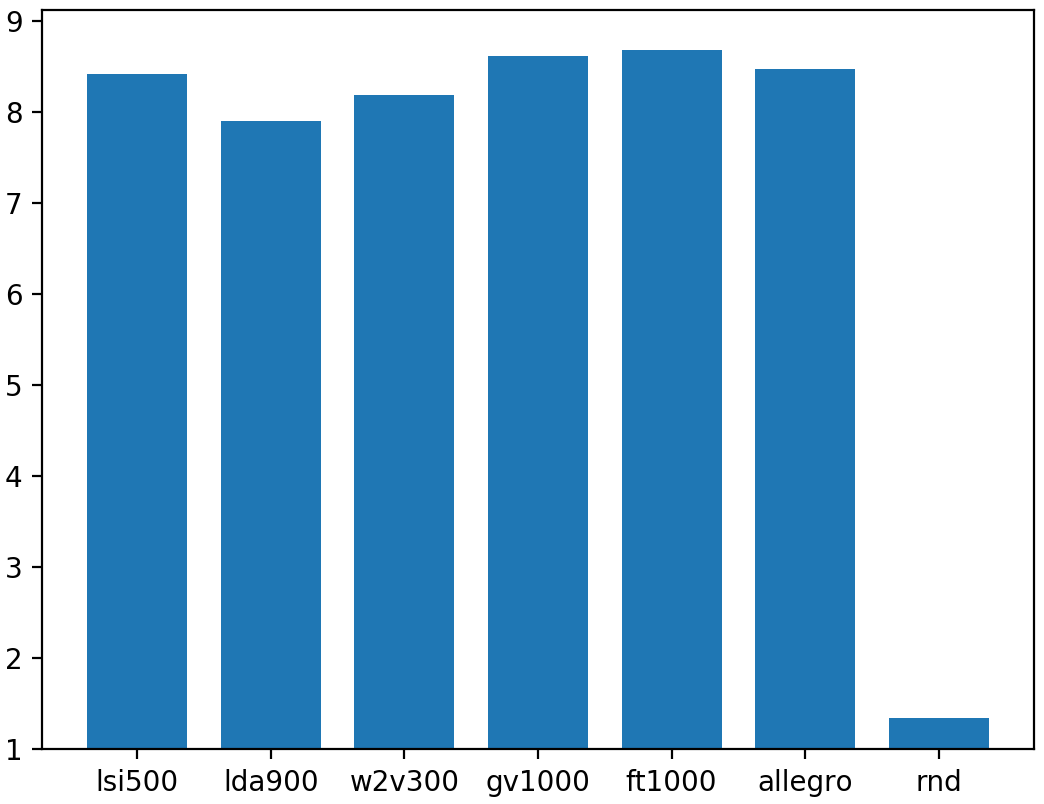
\includegraphics[width=0.45\textwidth]{results.png}
		\caption{}
		%\label{fig:warstwy}
	\end{figure}
	
	Expert evaluation directly shows that none of the tested methods is significantly different
	from others. None of the tested adaptations of the methods of semantic text analysis does not depart as well
	from the current method used in Allegro. The difference between the best method (FastText)
	and the worst (LDA) is around 9%. Each of the tested methods also gave a significant result
	better than the random method.
	
	To answer the question posed at the beginning of this work, i.e. whether the semantic method
	Natural language analysis adapted to determine recommendations are in the state
	to match the quality of the current method used in Allegro, he performs the test he has
	to check whether there are grounds to believe that the results of any of the methods subjected
	expert judgment is detached statistically significantly from the rest of the tested methods.
	The statistical test that I carry out is the Kruskal-Wallis test. H0 accepts for the null hypothesis
	he equality of distributions of distributions in the populations from which the samples originated.
	In earlier tests, users assessed the similarity between the article and everyone
	from articles recommended for it, determined by evaluated methods. For data
	Kruskal-Wallis test entry accepts tests corresponding to test results for each
	from methods (except for the random method) submitted from the average assessment of users for the most relevant
	recommendations for each of the tested base articles.
	In the test, the level of significance is assumed? = 0.05. Finally, as a result of the Kruskal test
	Wallis receives p = 0.0571>? On the basis of which I state that there are no reasons to
	reject the null hypothesis - the difference between the quality of the recommendations of the tested methods is not
	56
	5.5. Test summary
	statistically significant. It means that neither of the tested semantic methods does not stick out
	from others, neither the previous Allegro method is significantly better / worse than others
	tested methods.
	
	
	\section{Conclusion}
	
	
	Comparison of the best configurations of the tested methods showed that there are no significant differences
	between methods of semantic text analysis adapted to the task of generating recommendations
	and the previous method used in Allegro based on the query for the Elasticsearch engine.
	
	
	After analyzing the test results
	you can answer: yes, each of the methods of semantic analysis of the natural language in yours
	the best configuration can be adapted to generate article recommendations
	based on the content of the article currently displayed by the user of the website. recommendations
	these in the opinion of users do not undermine the quality of the current method.
	Using the methods of semantic text analysis allows to capture the hidden similarities between
	documents, where the documents combine not the same words or synonyms, but some abstract ones
	concepts related to each other. An important advantage of semantic methods compared to the previous one
	the method used in Allegro is the fact that they are based only on content
	articles. This frees the authors of the articles from independently providing them with additional metatags,
	of which the current method is used to a large extent.
	
	
	\begin{thebibliography}{99}
		
		\bibitem[Figueredo and Wolf, 2009]{Figueredo:2009dg}
		Figueredo, A.~J. and Wolf, P. S.~A. (2009).
		\newblock Assortative pairing and life history strategy - a cross-cultural
		study.
		\newblock {\em Human Nature}, 20:317--330.
		
		
		\bibitem{allegro}
		Opis Allegro
		\url{https://magazyn.allegro.pl/3333-serwis-allegro-to-nasz-sposob-na-wasze-szybkie-i-wygodne-zakupy-przez-internet}
		(dostęp 07.05.2017)
		
		\bibitem{bengio}
		Y. Bengio, R. Ducharme, P. Vincent, C. Jauvin,
		\emph{A Neural Probabilistic Language Model},
		Journal of Machine Learning Research 3 1137–1155,
		2003
		
		\bibitem{lda}
		D. M. Blei, A. Y. Ng, M. I. Jordan,
		\emph{Latent Dirichlet Allocation},
		Journal of Machine Learning Research, tom 3 num. 4–5,
		2003
		
		\bibitem{aylien}
		Blog Aylien
		\url{http://blog.aylien.com/overview-word-embeddings-history-word2vec-cbow-glove/}
		(dostęp 18.08.2017)
		
		\bibitem{c_w}
		R. Collobert, J. Weston,
		\emph{A Unified Architecture for Natural Language Processing: Deep Neural Networks with Multitask Learning},
		NEC Labs America,
		2008
		
		\bibitem{engines}
		W. B. Croft, D. Metzler, T. Strohman,
		\emph{Search Engines. Information Retrieval in Practice},
		Pearson Education, Inc.,
		6-9,
		2015
		
		\bibitem{lsa}
		S. Deerwester, S. T. Dumais, G. W. Furnas, T. K. Landauer, R. Harshman,
		\emph{Indexing by latent semantic analysis},
		Journal of the American Society for Information Science, tom 41, num. 6,
		1990
		
		\bibitem{elastic}
		Elasticsearch
		\url{https://www.elastic.co/}
		(dostęp 18.08.2017)
		
		\bibitem{elastic_companies}
		Firmy korzystające z Elasticsearch
		\url{https://www.elastic.co/use-cases}
		(dostęp 10.08.17)
		
		\bibitem{firth}
		J.R. Firth,
		\emph{A synopsis of linguistic theory 1930-1955},
		Oxford: Philological Society,
		1957
		
		\bibitem{svd}
		G. H. Golub, W. Kahan,
		\emph{Calculating the singular values and pseudo-inverse of a matrix},
		Journal of the Society for Industrial and Applied Mathematics: Series B, Numerical Analysis. 2 (2),
		1965
		
		\bibitem{bow}
		Z. S. Harris,
		\emph{Distributional Structure},
		Word,
		10 (2/3): 146–62,
		1954
		
		\bibitem{google_word2vec}
		Informacje o Word2vec
		\url{https://code.google.com/archive/p/word2vec/}
		(dostęp 26.05.2017)
		
		\bibitem{ndcg}
		K. Jarvelin, J. Kekalainen,
		\emph{Cumulated gain-based evaluation of IR techniques},
		University of Tampere,
		2002
		
		\bibitem{fasttext}
		A. Joulin, E. Grave, P. Bojanowski T. Mikolov,
		\emph{Bag of Tricks for Efficient Text Classification},
		Facebook AI Research,
		2016
		
		\bibitem{pias}
		P. Kędzia, G. Czachor, M. Piasecki, J. Kocoń
		\emph{Vector representations of polish words (Word2Vec method)},
		Wrocław University of Technology,
		2016,
		\url{https://clarin-pl.eu/dspace/handle/11321/327}
		(dostęp 26.06.2017)
		
		\bibitem{wmd}
		M. J. Kusner, Y. Sun, N. I. Kolkin, K. Q. Weinberger,
		\emph{From Word Embeddings To Document Distances},
		International Conference on Machine Learning (ICML),
		2015
		
		\bibitem{lucene}
		Lucene
		\url{https://lucene.apache.org/}
		(dostęp 18.08.2017)
		
		\bibitem{word2vec}
		T. Mikolov, K. Chen, G. Corrado, J. Dean,
		\emph{Efficient Estimation of Word Representations in Vector Space},
		International Conference on Machine Learning (ICML),
		2013
		
		\bibitem{morfologik}
		Morfologik
		\url{http://morfologik.blogspot.com/}
		(dostęp 07.05.2017)
		
		\bibitem{glove_cran}
		Opis GloVe
		\url{https://cran.r-project.org/web/packages/text2vec/vignettes/glove.html}
		(dostęp 30.08.2017)
		
		\bibitem{word2vec_tutorial}
		Opis Word2vec
		\url{http://mccormickml.com/2016/04/19/word2vec-tutorial-the-skip-gram-model/}
		(dostęp 26.05.2017)
		
		\bibitem{emd_method}
		O. Pele, M. Werman,
		\emph{Fast and robust earth mover's distances},
		ICCV,
		2009
		
		\bibitem{glove}
		J. Pennington, R. Socher, C. D. Manning,
		\emph{GloVe: Global Vectors for Word Representation},
		Computer Science Department, Stanford University, Stanford, CA 94305,
		2014
		
		\bibitem{all_naj}
		Porównanie największych polskich serwisów aukcyjnych
		\url{http://gadzetomania.pl/11824,zakupy-w-sieci-porownanie-najwiekszych-polskich-serwisow-aukcyjnych-2}
		(dostęp 09.08.17)
		
		\bibitem{handbook}
		F. Ricci, L. Rokach, B. Shapira,
		\emph{Introduction to Recommender Systems Handbook},
		Springer,
		1-4,
		2011
		
		\bibitem{handbook_col}
		F. Ricci, L. Rokach, B. Shapira,
		\emph{Introduction to Recommender Systems Handbook},
		Springer,
		145-147,
		2011
		
		\bibitem{handbook_cb}
		F. Ricci, L. Rokach, B. Shapira,
		\emph{Introduction to Recommender Systems Handbook},
		Springer,
		73-75,
		2011
		
		\bibitem{emd}
		Y. Rubner, C. Tomasi, L. J. Guibas,
		\emph{The Earth Mover's Distance as a Metric for Image Retrieval},
		Computer Science Department, Stanford University,
		1,
		2000	
		
		\bibitem{tf_idf}
		G. Salton and M. McGill,
		\emph{Introduction to modern information retrieval},
		McGraw-Hill,
		1983
		
		\bibitem{stopwords}
		Słowa stopu w Wikipedii
		\url{https://pl.wikipedia.org/wiki/Wikipedia:Stopwords}
		(dostęp 15.04.2017)
		
		\bibitem{slownik}
		Słownik Języka Polskiego PWN
		\url{http://sjp.pwn.pl/sjp/artykul;2441396.html}
		(dostęp 07.05.2017)
		
		\bibitem{screen_allegro}
		Strona Allegro z artykułem
		\url{https://allegro.pl/artykul/jaka-farba-dla-alergika-55917/}
		(dostęp 26.06.2017)
		
		\bibitem{wordnet}
		Wordnet
		\url{http://plwordnet.pwr.wroc.pl/wordnet/}
		(dostęp 28.06.2017)
		
		
	\end{thebibliography}
	
	%----------------------------------------------------------------------------------------
	
\end{document}
.